\chapter{Diseño e implementación} % Main chapter title

\label{Chapter3} % Change X to a consecutive number; for referencing this chapter elsewhere, use \ref{ChapterX}

\definecolor{mygreen}{rgb}{0,0.6,0}
\definecolor{mygray}{rgb}{0.5,0.5,0.5}
\definecolor{mymauve}{rgb}{0.58,0,0.82}

%%%%%%%%%%%%%%%%%%%%%%%%%%%%%%%%%%%%%%%%%%%%%%%%%%%%%%%%%%%%%%%%%%%%%%%%%%%%%
% parámetros para configurar el formato del código en los entornos lstlisting
%%%%%%%%%%%%%%%%%%%%%%%%%%%%%%%%%%%%%%%%%%%%%%%%%%%%%%%%%%%%%%%%%%%%%%%%%%%%%
\lstset{ %
  backgroundcolor=\color{white},   % choose the background color; you must add \usepackage{color} or \usepackage{xcolor}
  basicstyle=\footnotesize,        % the size of the fonts that are used for the code
  breakatwhitespace=false,         % sets if automatic breaks should only happen at whitespace
  breaklines=true,                 % sets automatic line breaking
  captionpos=b,                    % sets the caption-position to bottom
  commentstyle=\color{mygreen},    % comment style
  deletekeywords={...},            % if you want to delete keywords from the given language
  %escapeinside={\%*}{*)},          % if you want to add LaTeX within your code
  %extendedchars=true,              % lets you use non-ASCII characters; for 8-bits encodings only, does not work with UTF-8
  %frame=single,	                % adds a frame around the code
  keepspaces=true,                 % keeps spaces in text, useful for keeping indentation of code (possibly needs columns=flexible)
  keywordstyle=\color{blue},       % keyword style
  language=[ANSI]C,                % the language of the code
  %otherkeywords={*,...},           % if you want to add more keywords to the set
  numbers=left,                    % where to put the line-numbers; possible values are (none, left, right)
  numbersep=5pt,                   % how far the line-numbers are from the code
  numberstyle=\tiny\color{mygray}, % the style that is used for the line-numbers
  rulecolor=\color{black},         % if not set, the frame-color may be changed on line-breaks within not-black text (e.g. comments (green here))
  showspaces=false,                % show spaces everywhere adding particular underscores; it overrides 'showstringspaces'
  showstringspaces=false,          % underline spaces within strings only
  showtabs=false,                  % show tabs within strings adding particular underscores
  stepnumber=1,                    % the step between two line-numbers. If it's 1, each line will be numbered
  stringstyle=\color{mymauve},     % string literal style
  tabsize=2,	                   % sets default tabsize to 2 spaces
  title=\lstname,                  % show the filename of files included with \lstinputlisting; also try caption instead of title
  morecomment=[s]{/*}{*/}
}


%----------------------------------------------------------------------------------------
%	SECTION 1
%----------------------------------------------------------------------------------------
\section{Autovalidación del dispositivo bajo prueba}
\label{sec:autovalidacion}

\begin{figure}[htbp]
	\centering
	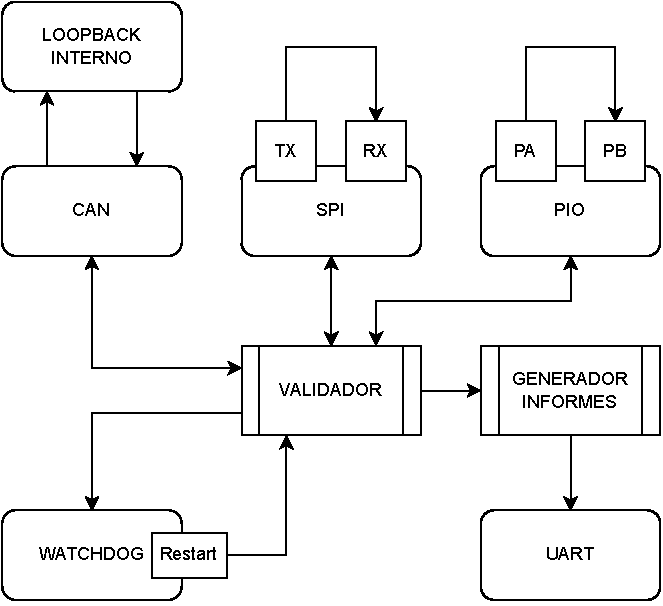
\includegraphics[width=0.8\textwidth]{./Figures/firmware_detallado.pdf}
    \caption{Diagrama en bloques del firmware de autovalidación.}
	\label{fig:firmwaredetail}
\end{figure}

\begin{figure}[htbp]
	\centering
	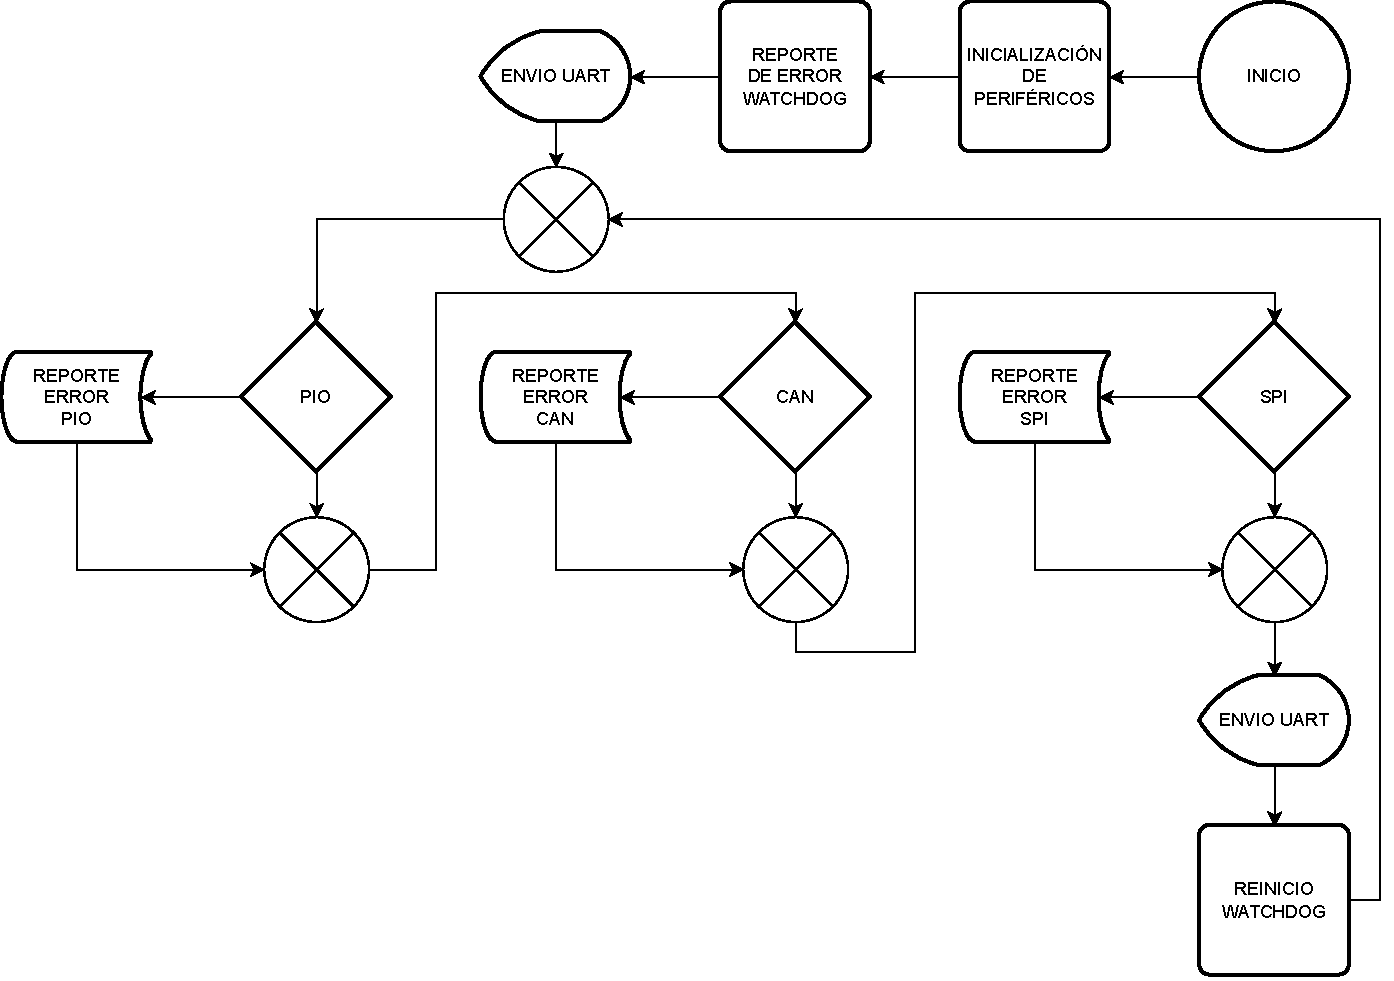
\includegraphics[width=\textwidth]{./Figures/firmwareflow.pdf}
    \caption{Flujo del firmware de autovalidación.}
	\label{fig:firmwareflow}
\end{figure}

\begin{figure}[htbp]
	\centering
	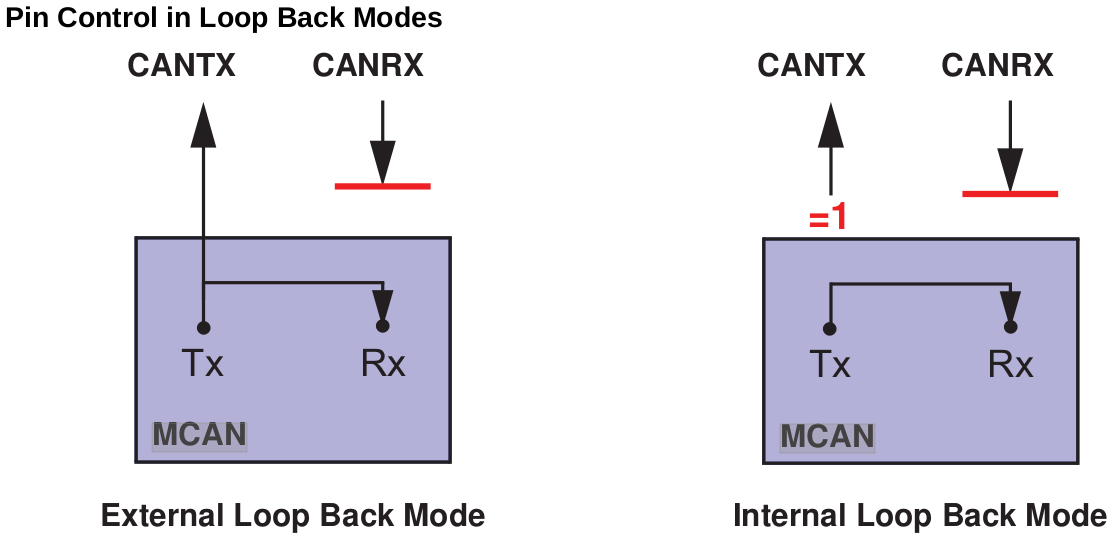
\includegraphics[width=0.8\textwidth]{./Figures/canloopback.png}
    \caption{Diagrama de \emph{loopback} del periférico CAN\citep{ARTICLE:dutdatasheet}.}
	\label{fig:canloopback}
\end{figure}

\begin{figure}[htbp]
	\centering
	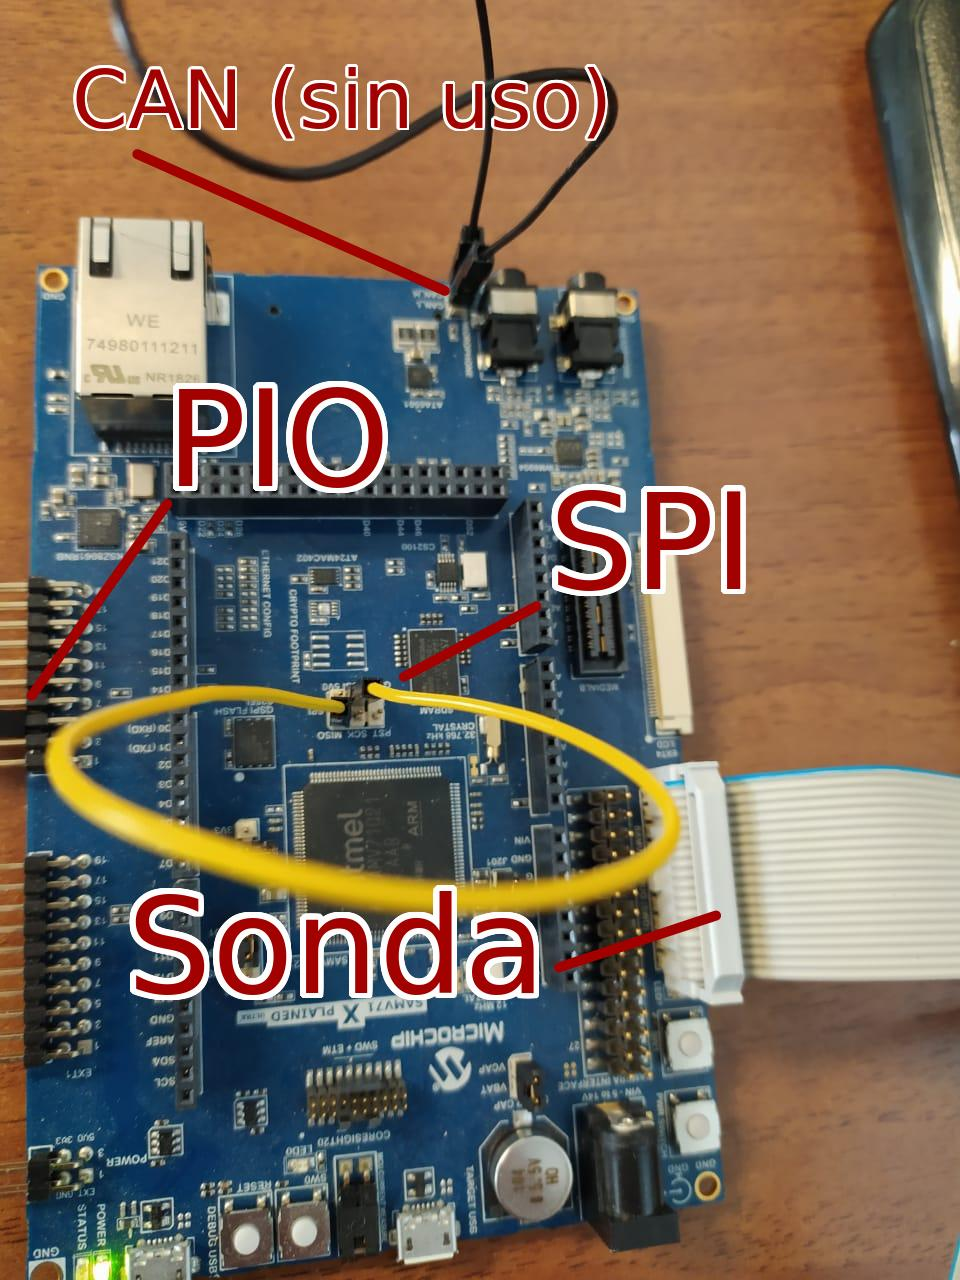
\includegraphics[width=0.8\textwidth]{./Figures/labo.jpeg}
    \caption{Fotografía del dispositivo bajo prueba.}
	\label{fig:labo}
\end{figure}

\begin{table}[h]
	\centering
	\caption[Estrategias de depuración]{Comparación entre estrategias de depuración}

	\begin{tabular}{l c c}    
		\toprule
        \textbf{Periférico} & \textbf{Validación}       & \textbf{Detección en un ciclo}\\
		\midrule
		CAN                 & Loopback interno          & Si\\		
		PIO                 & Loopback externo          & No\\
		SPI                 & Loopback externo          & Si\\
		UART                & Lógica en firmware        & No\\
		Watchdog            & Lógica en firmware        & No\\
		\bottomrule
		\hline
	\end{tabular}
	\label{tab:perifericos}
\end{table}
